\documentclass[addpoints]{exam}
\usepackage[utf8]{inputenc}
\usepackage{multicol}
\usepackage{graphicx}
\usepackage{amsmath}
\usepackage[a4paper,top=15mm, bottom=15mm, left=15mm, right=15mm]{geometry}
 
\begin{document}
 
\begin{center}
	\fbox{\fbox{\parbox{5.5in}{\centering Istituti Card. C. Baronio - Vicenza \\ Anno scolastico 2018/2019 \\ Compito di Matematica \\ Classe 3a-4a AFM}}}
\end{center}

\vspace{5mm}

\makebox[\textwidth]{Nome e Cognome:\enspace\hrulefill Data:\enspace\hrulefill}
 
\begin{questions}

\question[1] Nella seguente figura, indica un punto P sulla circonferenza e segna cosa si intende per coseno e seno di quel punto. Scrivi poi i valori di seno e coseno per i 4 punti principali

\begin{figure}[h!]
	\centering
	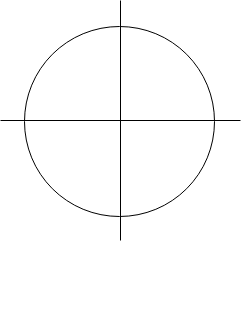
\includegraphics[scale=0.3]{SenoCoseno.png}
\end{figure}

\question[1] Quale tra queste è una parabola? Calcolane poi vertice e fuoco
\begin{checkboxes}
	\choice $y=3x+2$
	\choice $y=x^2-4x+2$
	\choice $x^2+y^2-2x+4y-4=0$
\end{checkboxes}

\question[1] Quale tra queste è una circonferenza? Calcolane poi centro e raggio
\begin{checkboxes}
	\choice $3x+5y=6$
	\choice $y=x^2-4x+2$
	\choice $x^2+y^2-2x+4y-4=0$
\end{checkboxes}

\question[2] Calcola il valore dei seguenti limiti, risolvendo eventuali forme indeterminate
	\begin{align*}
	\lim_{x \to -2} \frac{x+1}{x-3} \hspace{8mm}
	\lim_{x \to -3} \frac{x+6}{x+3} \hspace{8mm}
	\lim_{x \to \infty} \frac{x^2}{x} \hspace{8mm}
	\lim_{x \to \infty} \frac{3x-7}{5x+7} \hspace{8mm}
	\lim_{x \to \infty} \frac{x+3}{x^2-7} \hspace{8mm}
	\lim_{x \to -\infty} 6x^2-4x
	\end{align*}
	
	
\question[3] Calcola le seguenti derivate
	\begin{align*}
	D(1344) \hspace{8mm}
	D(45x) \hspace{8mm}
	D(2x^2) \hspace{8mm}
	D(\frac{4}{x}) \hspace{8mm}
	D(log(x)) \\
	D(log(3x^2)) \hspace{8mm}
	D(x^2+3x^3-2x) \hspace{8mm}
	D(x^2*log(x))
	\end{align*}
	
\question[1] Un'urna contiene 10 palline bianche, 15 nere, 20 blu e 25 rosse. Trovare la probabilità che una pallina estratta sia:
\begin{checkboxes}
	\choice bianca o nera 
	\choice blu o rossa
	\choice bianca, nera o blu
\end{checkboxes}

\question Risolvi i seguenti esercizi:
\begin{parts}
	\part[\half] Quanti numeri di 5 cifre posso scrivere usando solo 1, 3, 5, 7, 9 senza ripetizioni? E con ripetizioni?
	\part[\half] In quanti modi diversi 3 bambini possono spartirsi 7 caramelle?
\end{parts}

\end{questions}


\begin{center}
	\gradetable[h][questions]
\end{center}

\end{document}